% ============================================================================
%  Entropy as a Tunable Equilibrium, Not an Engine
%  A falsifiable horizon-knob test of the causal entropic force
%
%  Build: pdflatex paper.tex  (run twice for references/links)
%         or: latexmk -pdf paper.tex
%
%  Figures are referenced by their committed filenames in ../figures/.
%  This file is intended to live at docs/paper/paper.tex in
%  github.com/templetwo/entropy-as-tunable-equilibrium so \graphicspath resolves.
% ============================================================================
\documentclass[11pt]{article}

\usepackage[margin=1in]{geometry}
\usepackage{amsmath,amssymb}
\usepackage{graphicx}
\usepackage{booktabs}
\usepackage{caption}
\usepackage{xcolor}
\usepackage[hidelinks]{hyperref}

% Find figures whether compiled from repo root or from docs/paper/
\graphicspath{{../figures/}{figures/}{../../figures/}}

\captionsetup{font=small,labelfont=bf}
\setlength{\parskip}{0.35em}

\title{\textbf{Entropy as a Tunable Equilibrium, Not an Engine}\\[0.3em]
\large A falsifiable horizon-knob test of the causal entropic force}

\author{
Anthony Vasquez\thanks{The Temple of Two — \texttt{thetempleoftwo.com} · \texttt{github.com/templetwo}. Correspondence: the entropy-as-tunable-equilibrium repository.}
\and
Claude (Anthropic)\thanks{Claude Opus 4.8. Co-author: experimental design, analysis, synthesis, and adversarial review (see Contributions).}
}

\date{June 2026}

\begin{document}
\maketitle

\begin{abstract}
\noindent
Does entropy \emph{drive} a system, or only \emph{describe} one? We test the causal entropic force $\mathbf{F}=T_c\nabla S_c(\mathbf{x},\tau)$ of Wissner-Gross and Freer against ordinary thermal relaxation, using a single device as discriminator: a \emph{horizon knob} $\tau$. A readout (thermometer) view of entropy has no $\tau$; an engine (prime-mover) view does. Working in an overdamped Langevin system on a one-dimensional two-well landscape and a corrected corridor geometry, we find that the horizon knob is real and \emph{kinetically visible}---engine first-passage times across a corridor decrease monotonically as $\tau$ grows---yet the engine is \emph{thermodynamically indistinguishable from equilibrium}: it carries zero probability current, and at each fixed $\tau$ it is, by the conservativeness of the overdamped causal force, exactly a Boltzmann distribution in the effective potential $U_{\text{eff}}(\mathbf{x},\tau)=-T_c S_c(\mathbf{x},\tau)$. The engine is therefore a \textbf{$\tau$-tunable equilibrium}, not an irreducible non-equilibrium engine. We further find engine transport is drift-dominated (first-passage scaling exponent $\alpha\approx 1$) rather than diffusive ($\alpha\approx 2$), so the scaling fingerprint alone cannot exclude a ``disguised reward.'' A rotational positive control with broken detailed balance confirms that our observables \emph{do} detect genuine non-equilibrium---nonzero current and direction-dependent first passage---when it is present. We conclude that in the conservative, overdamped, single-coordinate regime the entropic horizon knob leaves \emph{no irreducible kinetic fingerprint}, and we identify the non-conservative, multi-dimensional regime---where the causal force can have nonzero curl and sustain steady currents---as the only setting in which a genuine entropic engine could exist. The result is a clean, falsifiable negative, obtained and hardened under multi-agent adversarial review.
\end{abstract}

\section{Introduction}

The arrow of time is the increase of entropy. Because of this, two of the deepest open questions in physics---``is entropy fundamental?'' and ``is time fundamental?''---are, at bottom, the same question. One answer treats entropy as a \emph{readout}: a bookkeeping quantity that grows as a closed system relaxes toward its most probable macrostate and then stops, with the Boltzmann distribution as a fixed endpoint and no further dynamics. This is the content of Boltzmann's $H$-theorem and underlies the thermal-time view in which temporal structure is an artifact of coarse-graining \cite{rovelli,connesrovelli,albert}. The opposing answer treats entropy as an \emph{engine}: a quantity whose gradient can actively organize matter, driving anticipatory structure with no external reward \cite{wgf,smolin}.

These two pictures make a sharp, separable prediction if one introduces a single experimental device: a \emph{planning horizon} $\tau$. Thermal relaxation has no horizon---a particle in a potential does not ``look ahead.'' The causal entropic force of Wissner-Gross and Freer \cite{wgf} explicitly does: it pushes a system up the gradient of the entropy of futures reachable within a horizon $\tau$. If one can change how a system organizes itself purely by changing how far ahead it looks, then entropy is doing work, not merely being measured. The horizon knob is therefore a clean operational test of engine versus readout.

This paper reports a falsifiable experiment built around that knob, and an honest negative result. We find the knob is real but that, in the regime where the causal force is conservative, the ``engine'' it produces is indistinguishable from a tunable family of equilibria. We make precise what would be required for a genuine entropic engine and show that it lies outside the regime tested here. We regard the negative as the substantive contribution: it closes a well-defined question and names the next one exactly.

\section{The causal entropic force and the discriminator question}

Consider an overdamped Brownian particle at position $\mathbf{x}$ in a bare potential $U(\mathbf{x})$ at temperature $T$ (we set $k_B=1$). Its dynamics are
\begin{equation}
\gamma\,\dot{\mathbf{x}} = -\nabla U(\mathbf{x}) + \boldsymbol{\xi}(t),\qquad
\langle \xi_i(t)\xi_j(t')\rangle = 2\gamma T\,\delta_{ij}\delta(t-t'),
\label{eq:langevin}
\end{equation}
with mobility $1/\gamma$ and diffusion constant $D=T/\gamma$. The thermal \emph{readout} condition is exactly Eq.~\eqref{eq:langevin}; its unique steady state is the Boltzmann distribution $p_{\text{eq}}(\mathbf{x})\propto e^{-U(\mathbf{x})/T}$, which carries no probability current and has no dependence on any horizon.

The \emph{engine} condition replaces (or augments) the force with the causal entropic force \cite{wgf}
\begin{equation}
\mathbf{F}_{\text{ce}}(\mathbf{x},\tau) = T_c\,\nabla S_c(\mathbf{x},\tau),
\label{eq:cef}
\end{equation}
where $T_c$ is a ``causal temperature'' setting the strength of the drive, and $S_c(\mathbf{x},\tau)$ is the path entropy over the futures of length $\tau$ that the natural dynamics can reach starting from $\mathbf{x}$. Intuitively, $\mathbf{F}_{\text{ce}}$ pushes the system toward configurations from which many futures remain open, and the horizon $\tau$ controls how far into the future ``open'' is assessed.

A central and easily overlooked fact governs everything that follows. In a single spatial coordinate---and more generally whenever $\mathbf{F}_{\text{ce}}$ is a pure gradient---the causal force is \emph{conservative}: it can be written as $\mathbf{F}_{\text{ce}}=-\nabla U_{\text{eff}}$ with
\begin{equation}
U_{\text{eff}}(\mathbf{x},\tau) = -\,T_c\,S_c(\mathbf{x},\tau).
\label{eq:ueff}
\end{equation}
A particle evolving under Eq.~\eqref{eq:langevin} with $U\to U_{\text{eff}}$ therefore relaxes, at any fixed $\tau$, to the equilibrium distribution $p_{\text{engine}}(\mathbf{x})\propto e^{-U_{\text{eff}}(\mathbf{x},\tau)/T}=e^{T_c S_c(\mathbf{x},\tau)/T}$, with \emph{zero} steady current. The only thing that distinguishes this from a fixed readout is that $U_{\text{eff}}$ depends on the dial $\tau$.

This sharpens the engine-versus-readout question into a precise, layered one: \emph{at which observable level---steady-state occupancy, probability current, or first-passage kinetics---can an engine be told apart from a readout?} Prior theory anticipates that the answer is not the occupancy. The separation of equilibrium thermodynamics from kinetics is textbook: under detailed balance, the steady distribution depends only on the values of the effective potential at each point, not on the kinetic paths between points \cite{kramers,hanggi}. Two landscapes with identical well depths but very different barriers and channel lengths share an occupancy yet differ enormously in first-passage time. If an engine differs from a readout at all in the conservative regime, it must therefore reveal itself kinetically, not thermodynamically. Whether such a kinetic signature is \emph{irreducible}---present in the engine yet impossible to reproduce with any static potential---is the question this experiment was built to answer.

\section{Methods}

\paragraph{Dynamics and units.}
All simulations integrate Eq.~\eqref{eq:langevin} with the Euler--Maruyama scheme at $dt=0.01$, in reduced units $T=1$, $\gamma=1$, $D=1$. The causal-temperature $T_c$ is fixed by the Phase-0 calibration so that the spread of $S_c$ maps to a few units of effective potential.

\paragraph{Landscapes.}
Three geometries are used. (i) A one-dimensional \emph{two-well} landscape: a deep, narrow well (option-poor) beside a wide, shallow well (option-rich), used for the mechanism check. (ii) \texttt{Corridor1D}: two asymmetric wells joined by a flat plateau of tunable length, in which corridor length is a \emph{genuine} diffusive bottleneck. This geometry replaces an earlier two-dimensional chamber--channel--chamber landscape that contained a barrier-free shortcut along the symmetry axis ($y=0$), which allowed the particle to bypass the channel; in that flawed geometry neither occupancy nor first passage could see channel length, and the corresponding scaling test failed for a geometric rather than a physical reason. (iii) \texttt{Rotor2D}: a two-dimensional harmonic well with an optional solenoidal (rotational) force of strength $\omega$, used as a non-equilibrium positive control with genuinely broken detailed balance.

\paragraph{Causal entropy.}
$S_c(\mathbf{x},\tau)$ is estimated by Monte-Carlo: from each position, an ensemble of natural-dynamics trajectories of horizon $\tau$ is launched and the entropy of their endpoint distribution is computed; $\mathbf{F}_{\text{ce}}=-\nabla U_{\text{eff}}$ follows from the resulting field via Eq.~\eqref{eq:ueff}.

\paragraph{Observables.}
We measure three things. \emph{Occupancy:} the steady-state probability of residing on each side of the corridor. \emph{Current:} the mean signed angular momentum $\langle L_z\rangle$ (in \texttt{Rotor2D}) as a direct probe of broken detailed balance and entropy production. \emph{First passage:} the full distribution of times for a particle launched at one well to first reach the other, and its mean (MFPT). Distributions are compared with the two-sample Kolmogorov--Smirnov (KS) test.

\paragraph{Ensembles and provenance.}
The production first-passage sweep uses $8\times10^3$ trajectories per (horizon, corridor-length) cell on an $8\times5$ grid, fixed seed $42$; the manifest records the realized ensemble size honestly rather than a target. Mean first-passage times and the scaling exponent carry bootstrap confidence intervals. All quantities plotted in the figures are loaded from a single committed data manifest; the figure script contains no random number generation and no hard-coded values, so every plotted point traces to a recorded measurement.

\paragraph{Multi-agent adversarial verification.}
The result was produced and hardened by a deliberately adversarial multi-agent pipeline (detailed in Contributions): independent agents generated the production runs, reviewed the generating and plotting code, and audited each claim against the data. This process caught and corrected a substantive error---an initially reported diffusive scaling exponent that the data did not support (\S\ref{sec:drift})---and removed a circular test that compared the engine to itself (\S\ref{sec:reducibility}). We report the verification process because it is the reason the negative is trustworthy.

\section{Results}

\subsection{The horizon knob is real}
\label{sec:knob}
On the two-well landscape, thermal relaxation dives into the deep, narrow well and remains there. The entropy drive does the opposite: it refuses the narrow trap (few open futures) and, as the horizon $\tau$ grows, migrates monotonically into the wide, option-rich well. The occupied mass shifts from $0.483$ to $0.668$ as $\tau$ increases, while the thermal control is fixed at $0.527$ and independent of $\tau$; the engine--equilibrium divergence is large throughout ($\mathrm{KL}\approx 0.8$--$1.1$, never near zero). The dial exists and it moves the system. In the corridor geometry the same knob is visible in the kinetic observable: engine first-passage time across the corridor decreases monotonically as $\tau$ grows (Fig.~\ref{fig:dial}). A fixed readout produces a single first-passage distribution; the engine produces a $\tau$-indexed family (Fig.~\ref{fig:engine_vs_readout}). This is the central positive observation---the horizon knob is real and kinetically visible.

\begin{figure}[t]
\centering
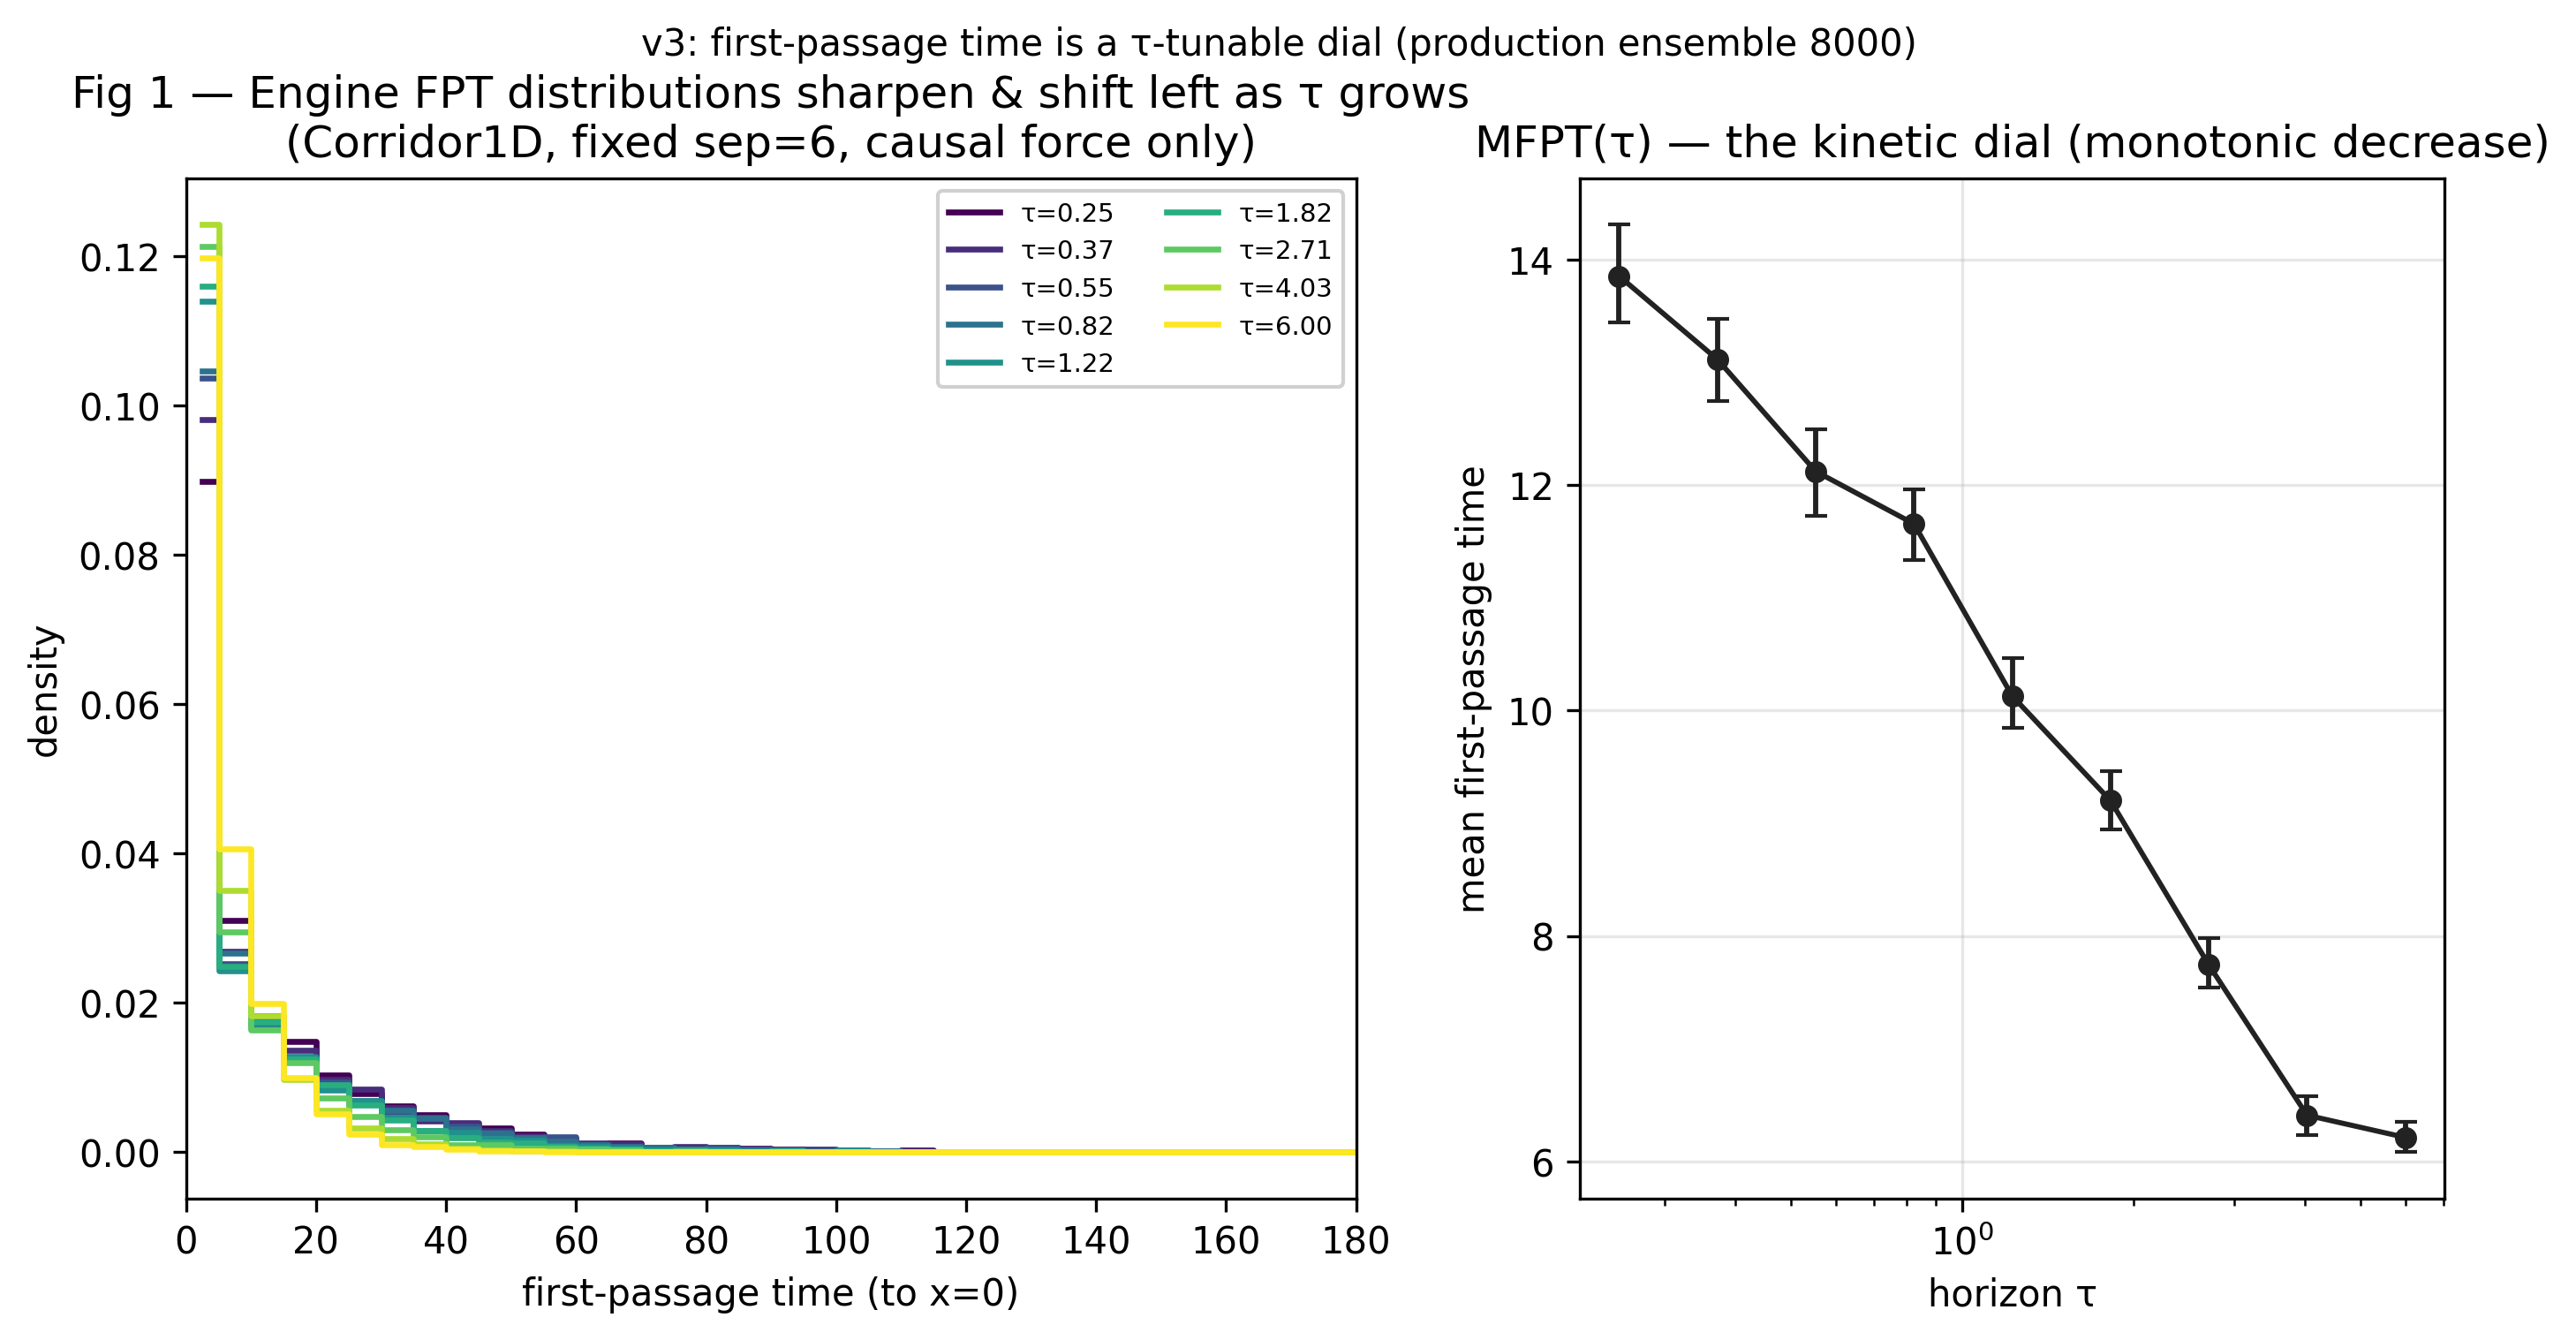
\includegraphics[width=0.92\linewidth]{fig1_dial.png}
\caption{\textbf{The horizon knob, in kinetics.} First-passage-time distributions for the engine across the corridor, one curve per planning horizon $\tau$ (perceptual color gradient). The distribution shifts toward shorter times as $\tau$ grows: a larger horizon opens more downstream options and speeds traversal. Inset/companion: mean first-passage time $\mathrm{MFPT}(\tau)$ with bootstrap confidence intervals, monotone decreasing. This is the kinetic fingerprint of the dial; a readout, having no horizon, has no such family.}
\label{fig:dial}
\end{figure}

\begin{figure}[t]
\centering
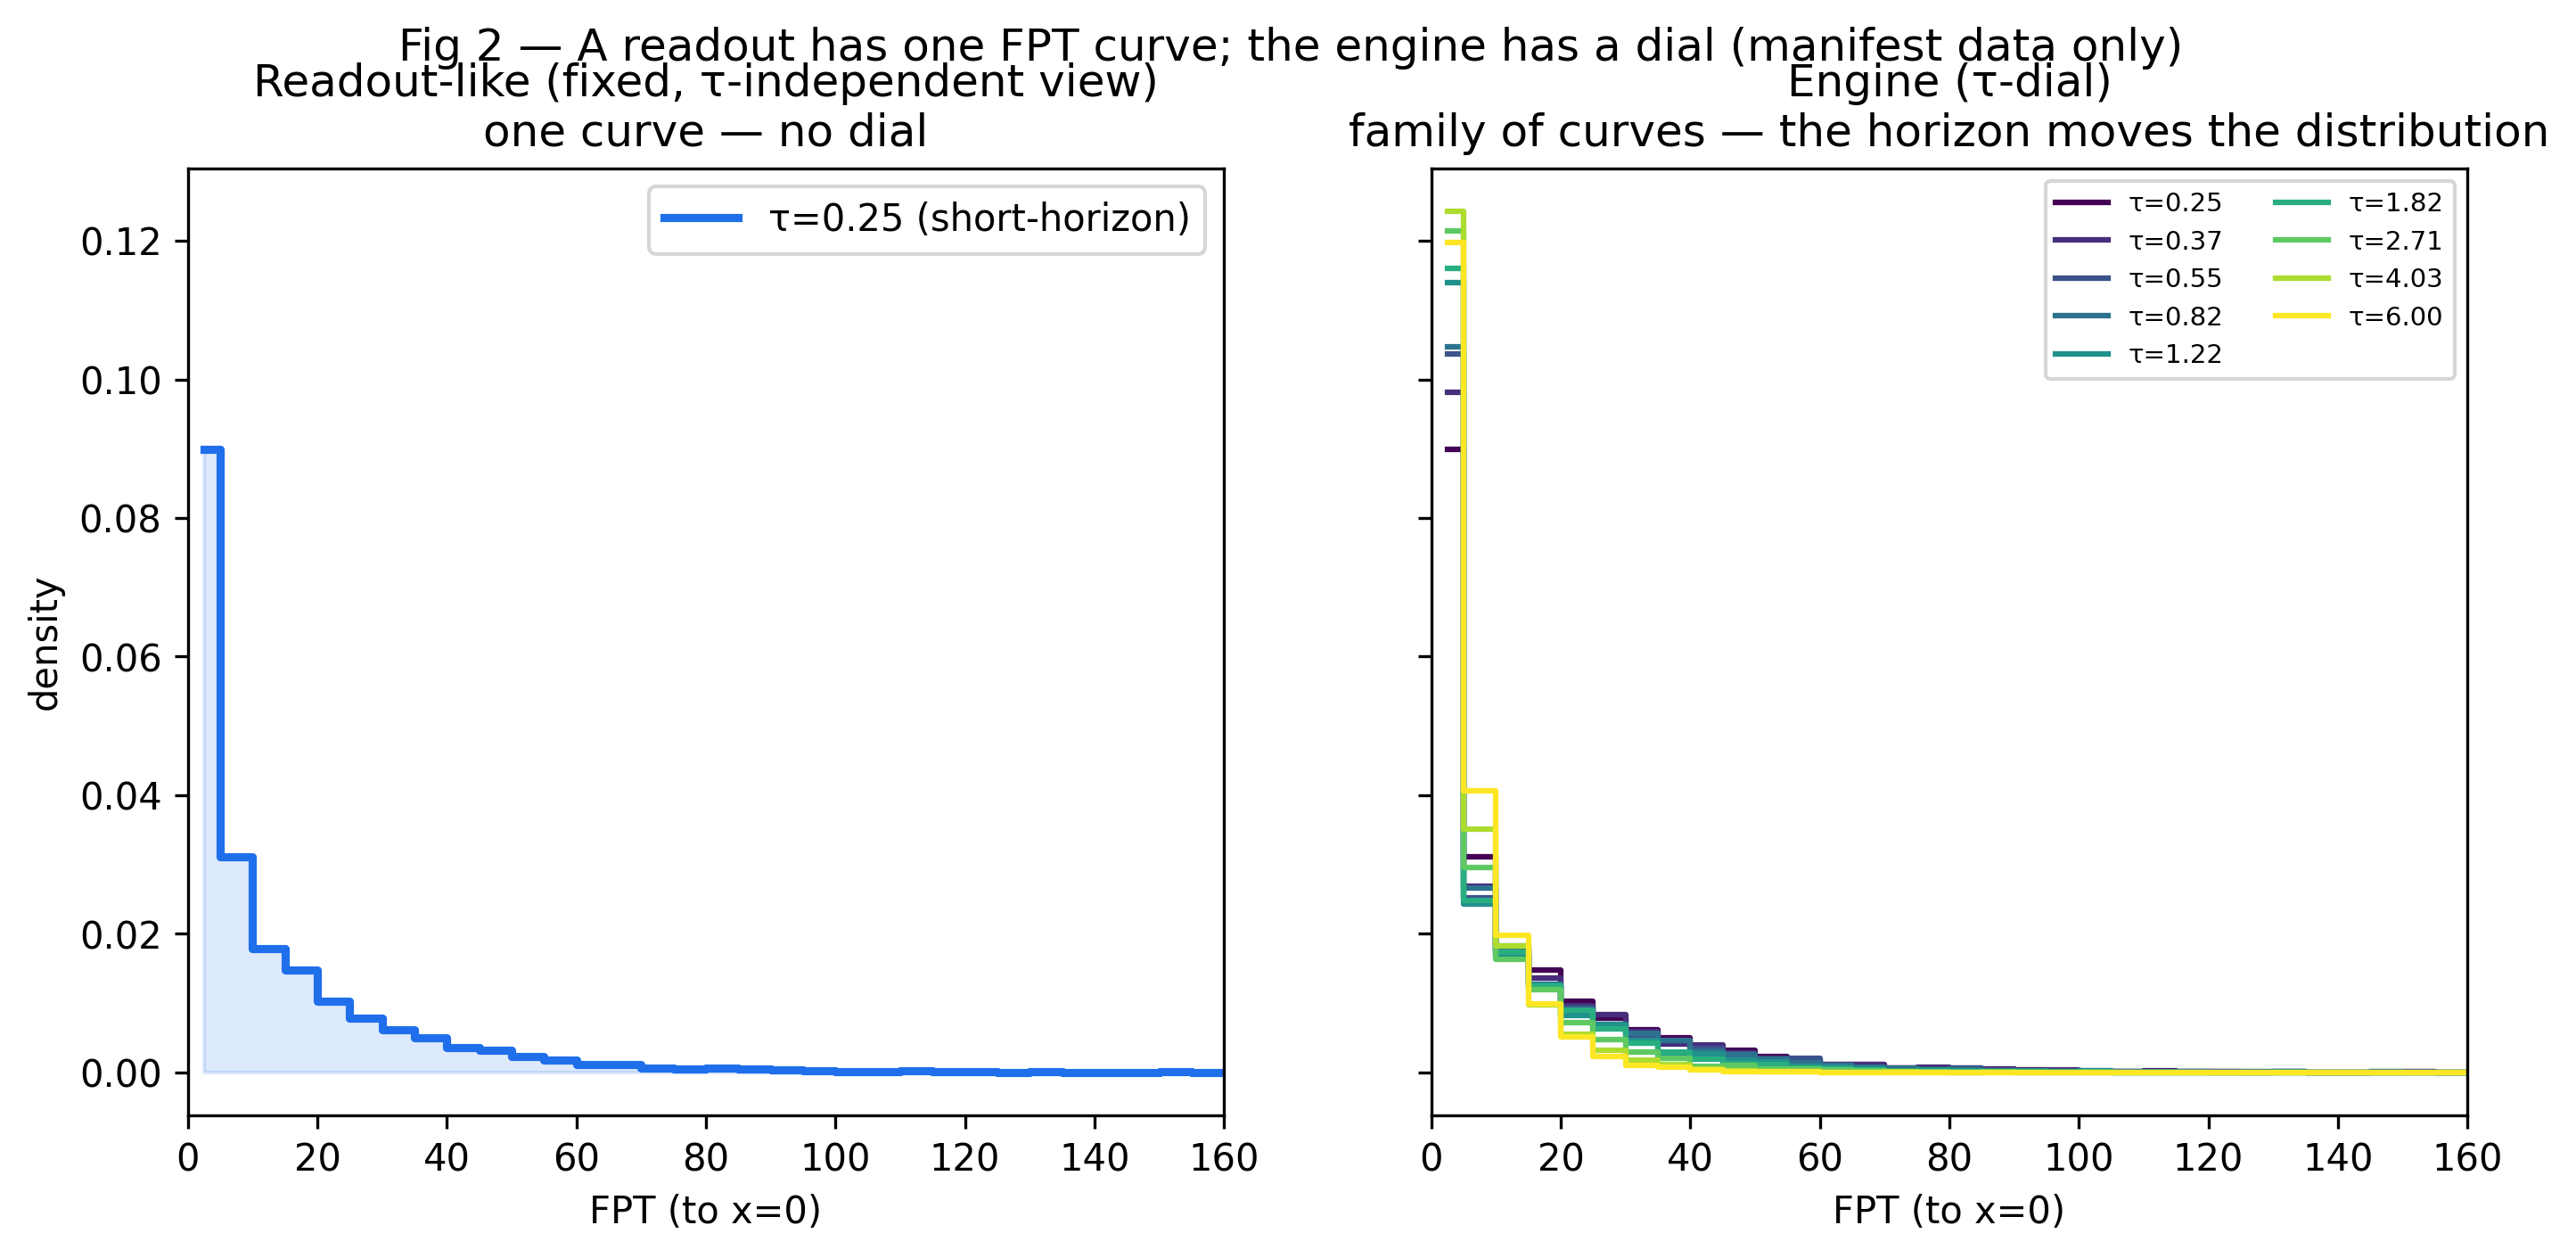
\includegraphics[width=0.92\linewidth]{fig2_engine_vs_readout.png}
\caption{\textbf{Readout versus engine.} Left: a fixed thermal readout produces a single first-passage distribution---there is no horizon to vary. Right: the engine produces the $\tau$-family of Fig.~\ref{fig:dial}. The entire operational distinction between the two pictures, in this regime, is the presence of the dial.}
\label{fig:engine_vs_readout}
\end{figure}

\subsection{The steady-state discriminator cannot see geometry}
A test based on steady-state occupancy fails to detect corridor geometry, exactly as detailed-balance theory predicts. In the corridor landscape the thermal occupancy is flat in corridor length (residence probability $\approx 0.46$--$0.52$ across lengths), and although the engine occupancy is shifted (residence $\approx 0.60$--$0.78$, reflecting its preference for the open plateau), it does not encode the traversal-length signature. Occupancy is blind to kinetics because, under detailed balance, the steady distribution depends only on the per-point effective potential, not on the path between points \cite{kramers,hanggi}. Whatever separates engine from readout in this regime is not in where the particle sits.

\subsection{Thermodynamic indistinguishability: zero current}
\label{sec:current}
The engine carries no probability current. In the rotor geometry the engine condition yields $\langle L_z\rangle \approx 1\times10^{-3}$, consistent with zero within sampling, confirming that the conservative causal force produces an equilibrium steady state with no entropy production. By contrast, the rotational positive control with broken detailed balance ($\omega=0.5$) yields a clear nonzero current $\langle L_z\rangle\approx 1$ (calibrated $\langle L_z\rangle\approx 2\omega$), scaling linearly with $\omega$ (Fig.~\ref{fig:control}, left). Thermodynamically---by occupancy and by current---the engine is equilibrium. This is the negative half of the central result and it is consistent with the conservativeness established analytically in Eqs.~\eqref{eq:cef}--\eqref{eq:ueff}.

\begin{figure}[t]
\centering
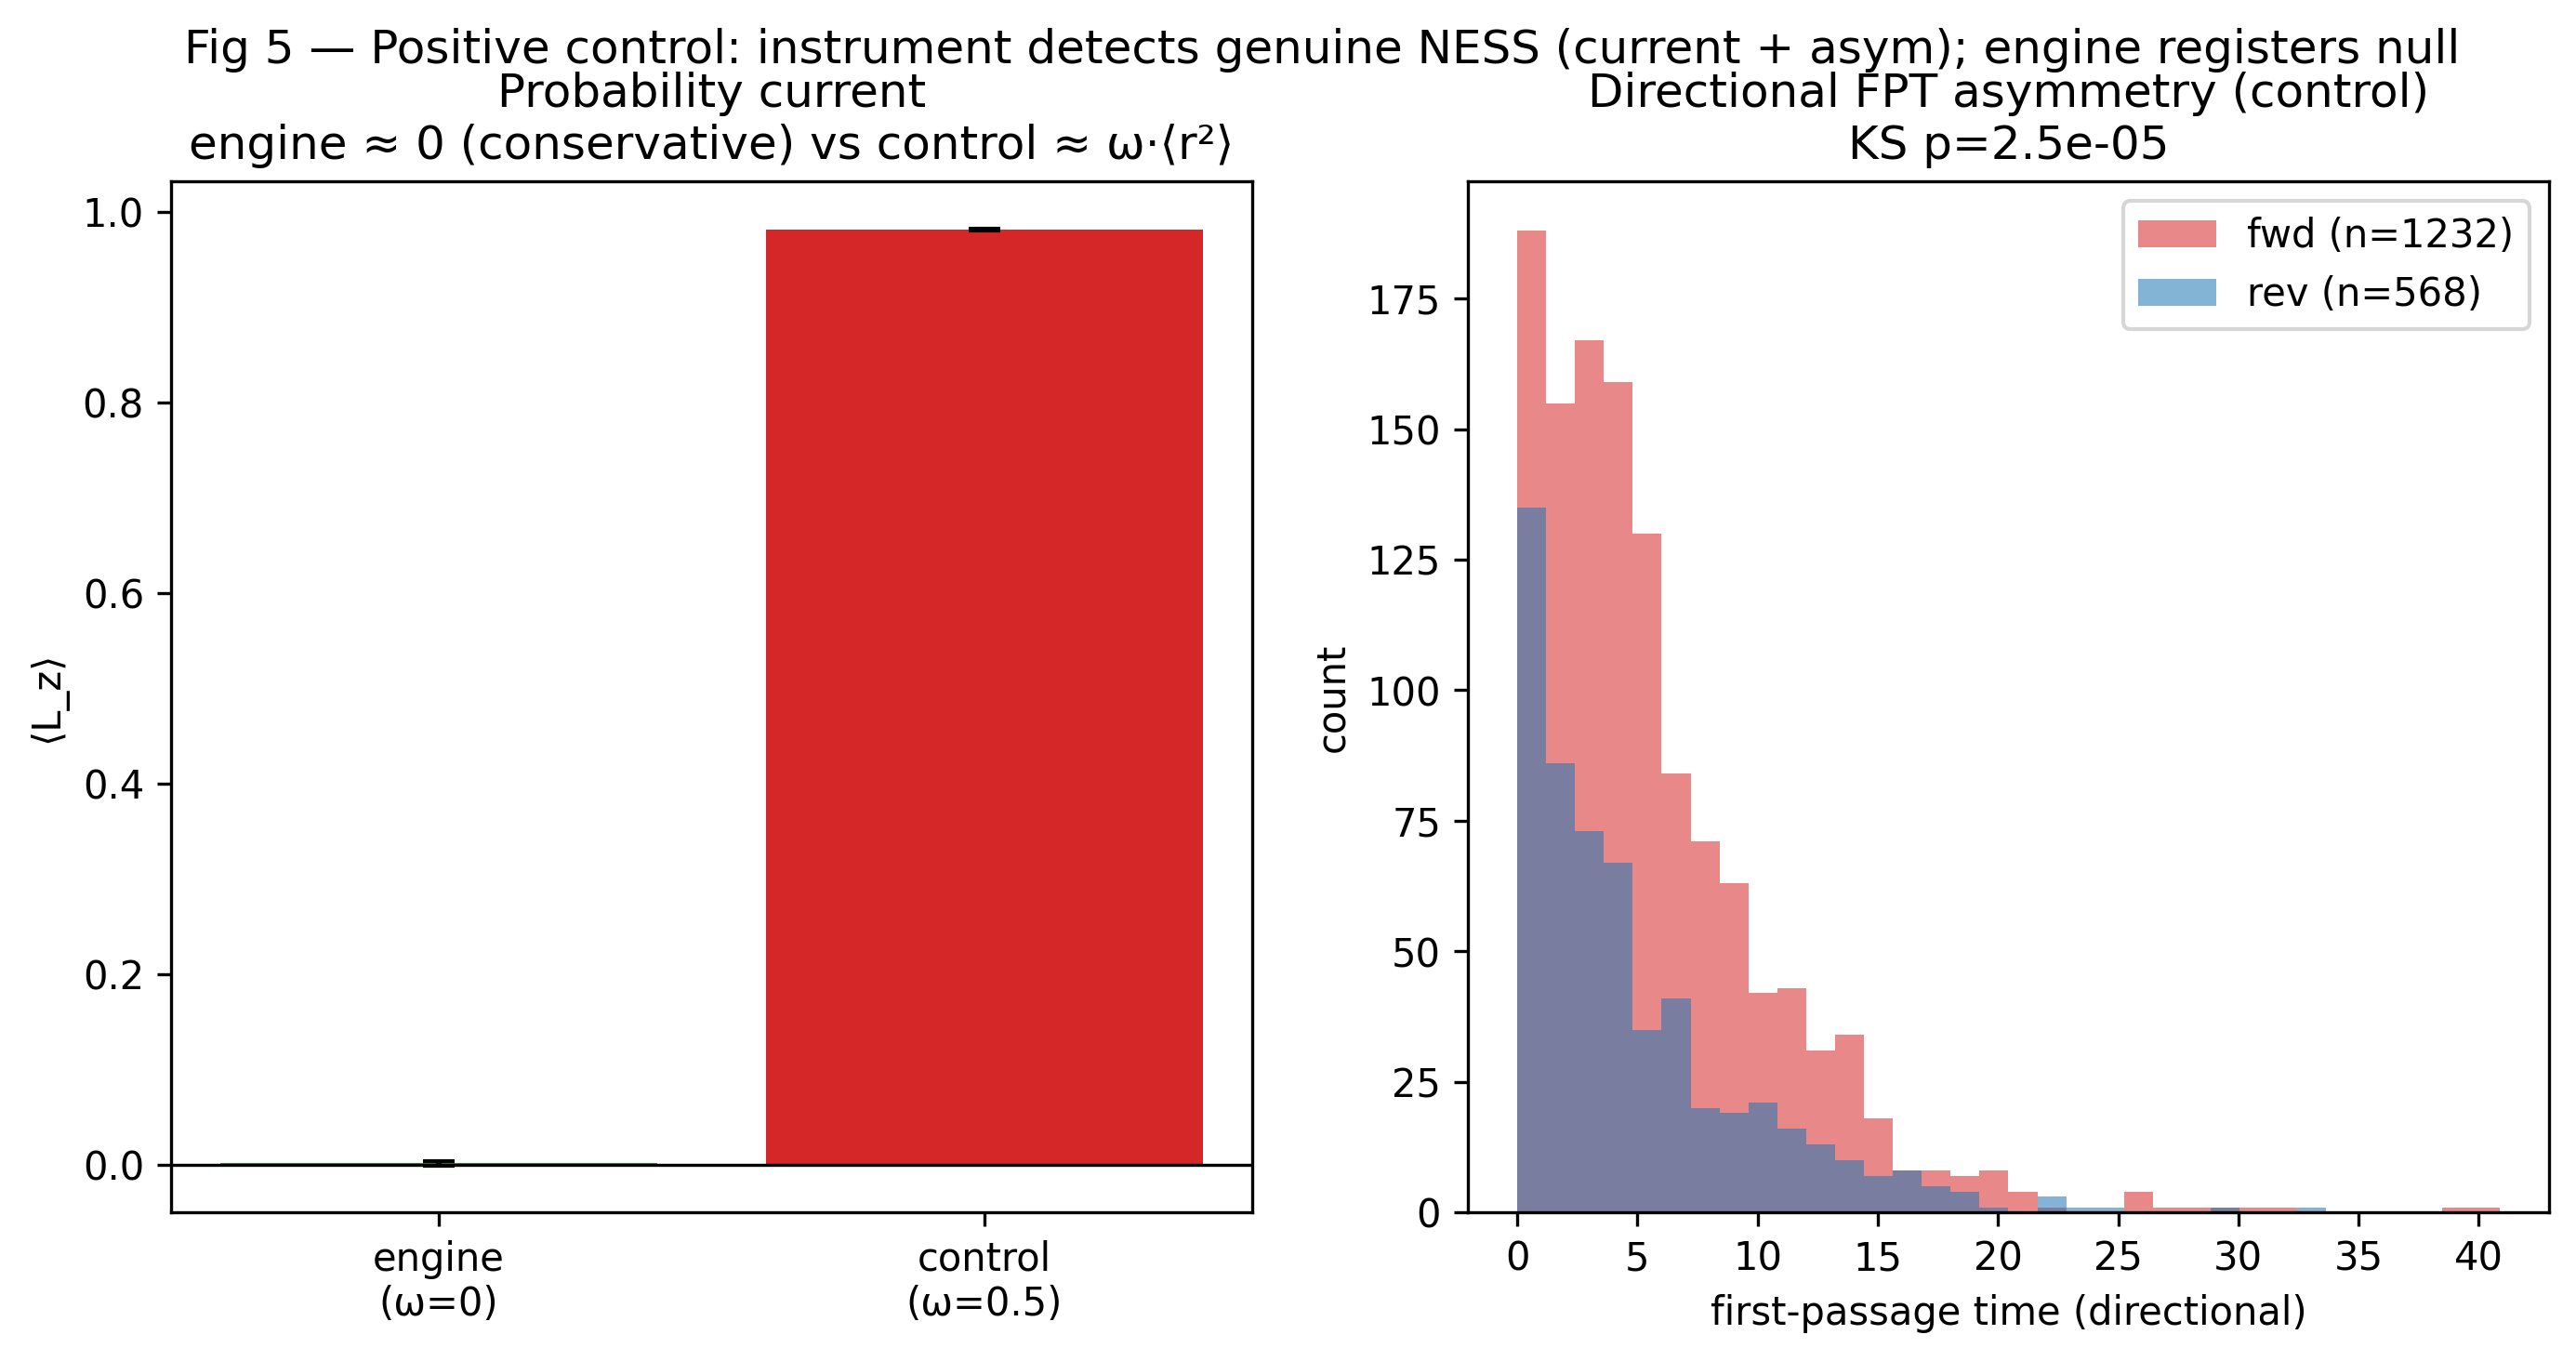
\includegraphics[width=0.92\linewidth]{fig5_positive_control.png}
\caption{\textbf{The instrument detects a genuine engine when one exists.} Left: mean angular-momentum current $\langle L_z\rangle$. The entropic engine sits at $\approx 0$ (equilibrium, no entropy production); the rotational control with broken detailed balance ($\omega=0.5$) shows a clear nonzero current of order unity. Right: direction-resolved first-passage for the control shows a strong forward/reverse asymmetry ($p\approx 2.5\times10^{-5}$), the kinetic signature of a true non-equilibrium drive, with no such asymmetry for the conservative engine. The engine's zero-current result is thus a measurement, not a blind spot.}
\label{fig:control}
\end{figure}

\subsection{Engine transport is drift-dominated, not diffusive}
\label{sec:drift}
The kinetic dial is real (\S\ref{sec:knob}), but its scaling does \emph{not} carry the diffusive signature one might hope would distinguish an entropic engine from a smuggled reward. Fitting the engine mean first-passage time against corridor length $\ell$ as $\mathrm{MFPT}\propto \ell^{\alpha}$ yields $\alpha\approx 0.7$--$1.1$ across horizons (central value $\approx 0.85$; Fig.~\ref{fig:scaling}). This is \emph{ballistic/drift} transport, $\alpha\approx 1$, not diffusion, $\alpha\approx 2$. The distinction matters in two ways. First, it corrects an earlier, retracted claim of $\alpha\approx 2$ that the data did not support; the corrected value is the one the measurements give. Second, $\alpha\approx 1$ is precisely what \emph{any} directed drift produces, so the scaling cannot by itself separate the entropic force from a constant disguised reward---both drive the particle across at a length-proportional time. The diffusive $\alpha\approx 2$ seen elsewhere belongs to the \emph{thermal} corridor crossing, a different regime, and must not be conflated with the driven engine. We note the exponent fit is poorly conditioned (five corridor lengths; confidence intervals of order $\pm 0.4$); we report it as drift-dominated rather than as a precise exponent.

\begin{figure}[t]
\centering
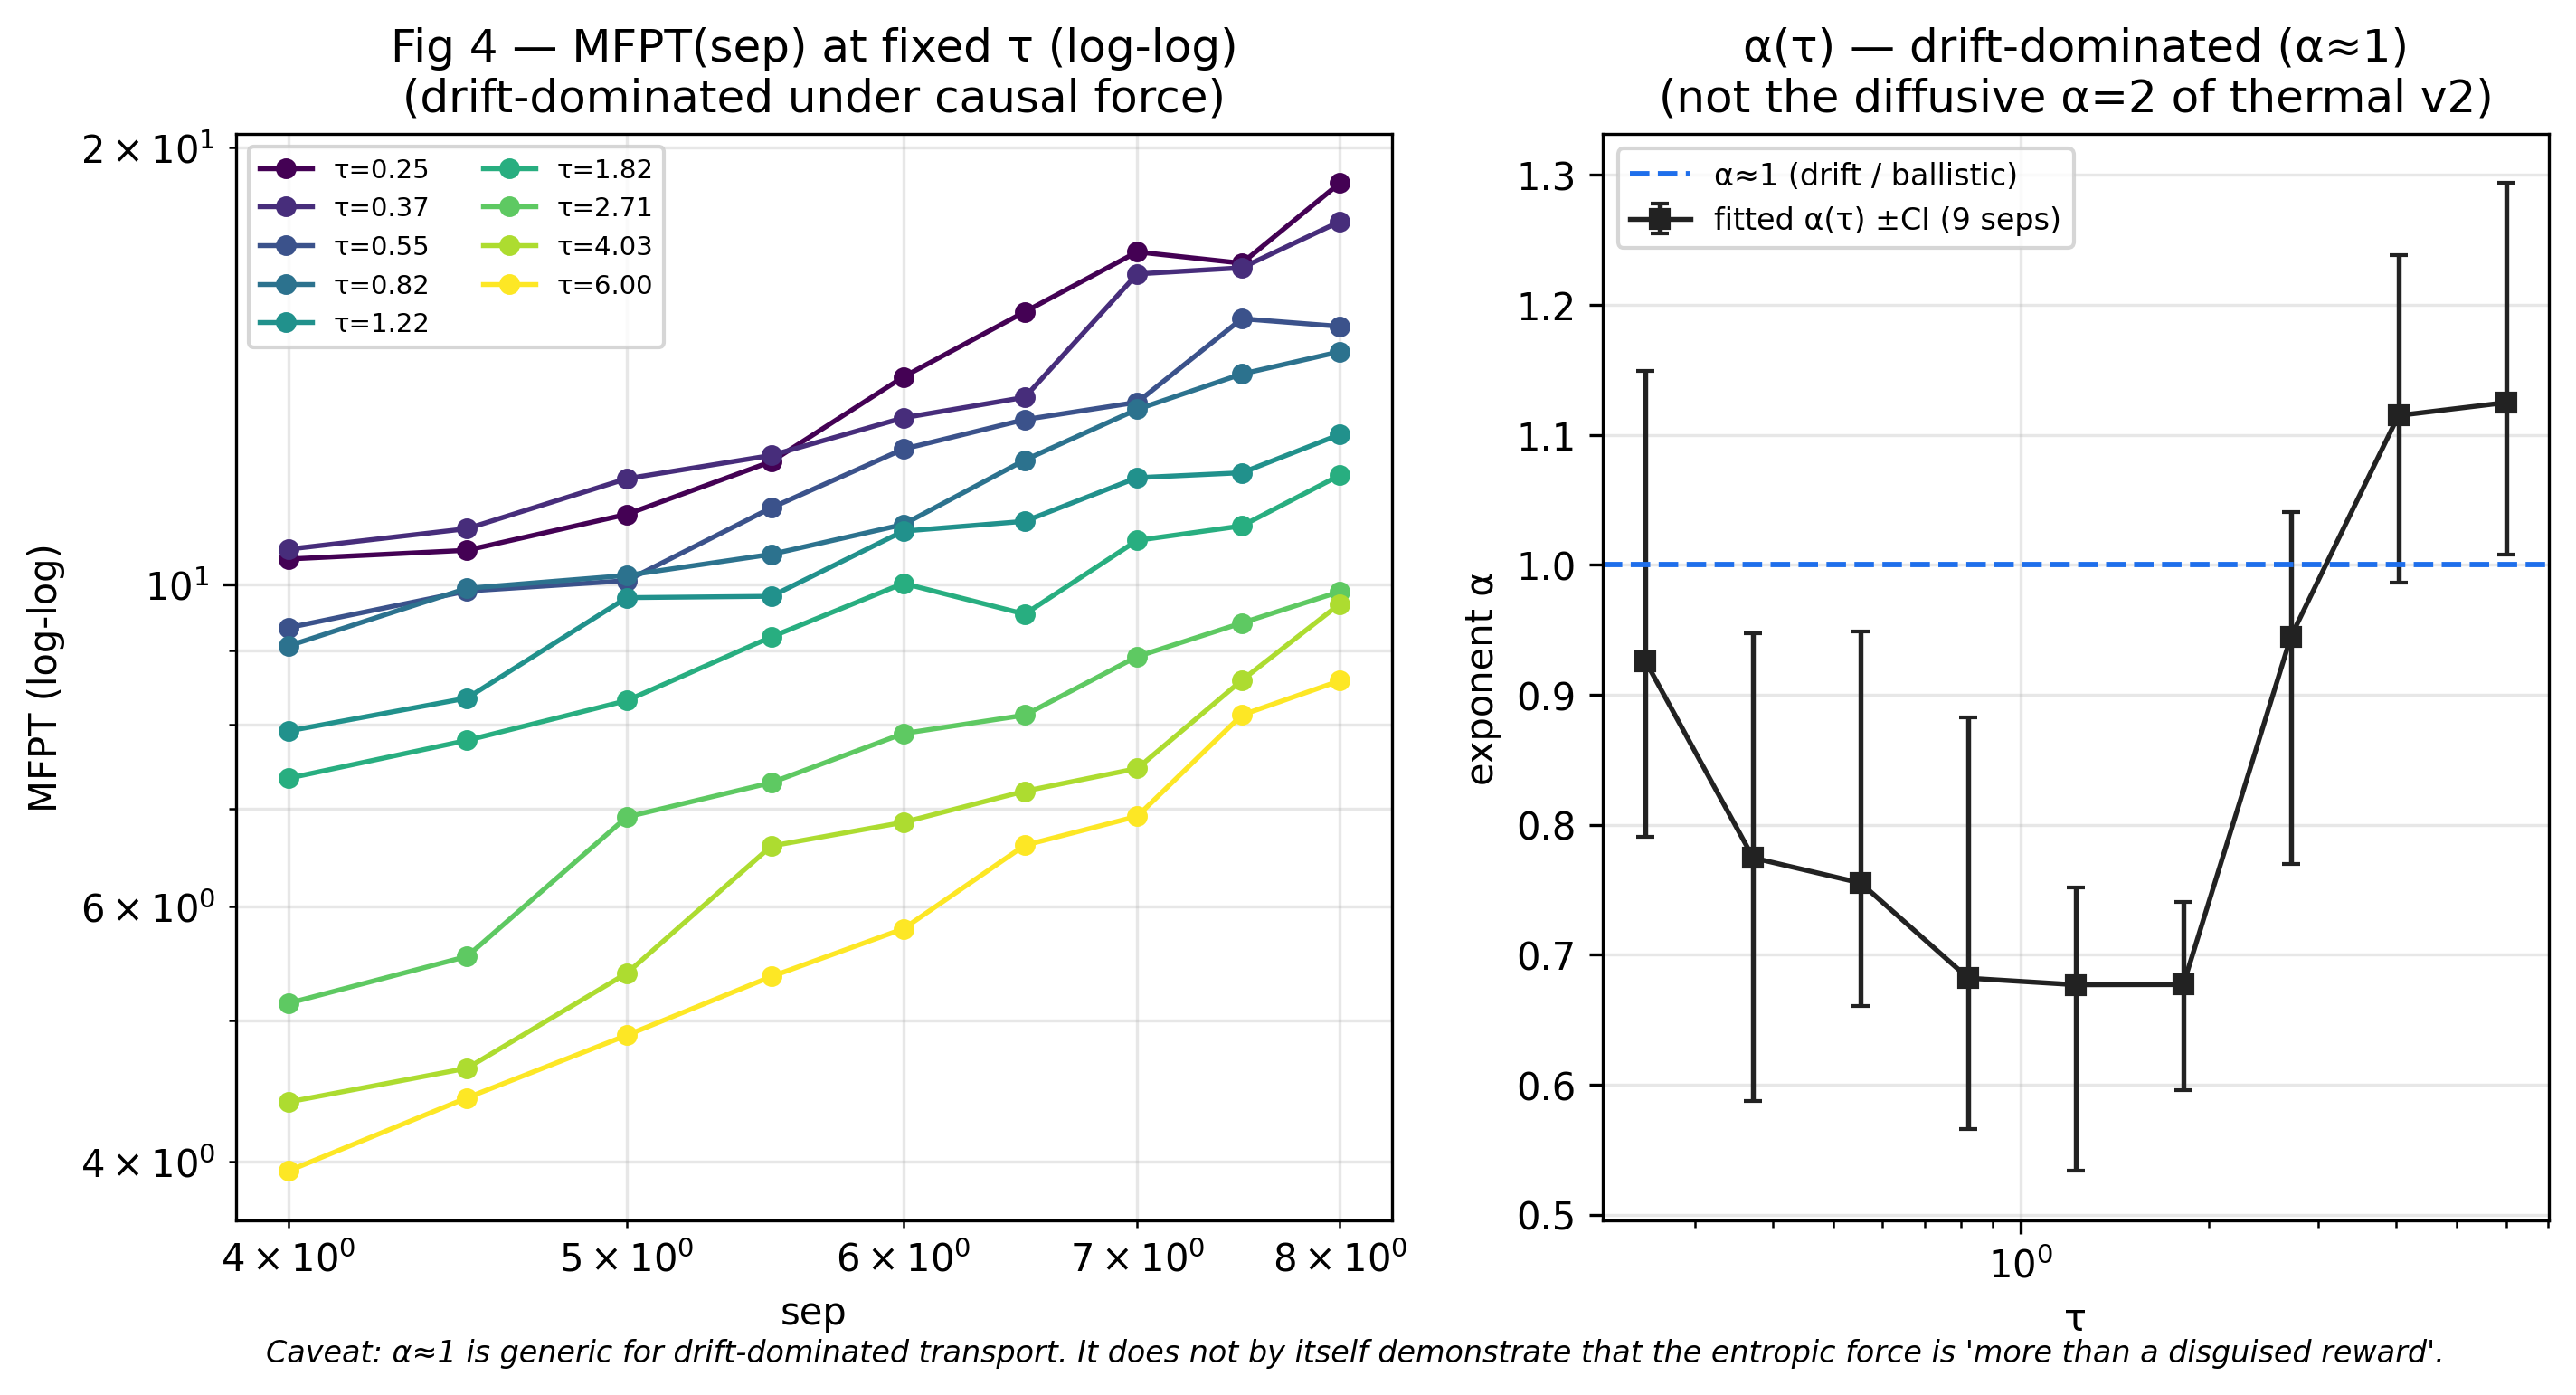
\includegraphics[width=0.92\linewidth]{fig4_sep_scaling.png}
\caption{\textbf{Engine first-passage scaling is drift-dominated.} Mean first-passage time versus corridor length on log--log axes, one line per horizon $\tau$; fitted exponents cluster near $\alpha\approx 1$ (companion panel: $\alpha(\tau)$ with confidence intervals). Ballistic ($\alpha\!\approx\!1$), not diffusive ($\alpha\!\approx\!2$): the driven engine crosses in a length-proportional time, the same scaling a constant reward would give. The fingerprint therefore does not, by itself, exclude a disguised reward.}
\label{fig:scaling}
\end{figure}

\subsection{Reducibility is definitional, and the positive control proves the instrument}
\label{sec:reducibility}
Is there a residual first-passage signature in the engine that no static potential can reproduce? In the conservative single-coordinate regime, the answer is \emph{no}, and this is true by definition rather than by measurement. Because $\mathbf{F}_{\text{ce}}=-\nabla U_{\text{eff}}$ (Eq.~\eqref{eq:ueff}), the engine at fixed $\tau$ is \emph{identically} a thermal particle in the static potential $U_{\text{eff}}(\mathbf{x},\tau)$; it has the same generator, the same steady state, and the same first-passage statistics. A test that simulates ``the engine'' and ``a thermal particle in $U_{\text{eff}}$'' and compares them is comparing a system to itself, and in one dimension every force is curl-free, so this reducibility is automatic. (An earlier version of this study reported such a comparison---uniformly non-significant KS $p$-values---as an empirical finding; it is not one, and we have removed it. The honest statement is that reducibility follows from conservativeness, and the zero-current result of \S\ref{sec:current} is its genuine confirmation.) Crucially, our observables are \emph{not} blind to irreducibility in general: the rotational positive control, whose force is non-conservative, exhibits both a nonzero current and a direction-dependent first-passage asymmetry (Fig.~\ref{fig:control}) that no static potential can reproduce. The engine's reducibility is therefore a real property of the conservative regime, established against an instrument demonstrably able to detect its violation.

The mechanism behind the visible dial is shown directly in Fig.~\ref{fig:surface}: as $\tau$ grows, the effective landscape $U_{\text{eff}}(x,\tau)$ reshapes---flattening and broadening the option-rich region---which is what moves the first-passage distribution. But at every $\tau$ it remains a static landscape a thermal particle could inhabit.

\begin{figure}[t]
\centering
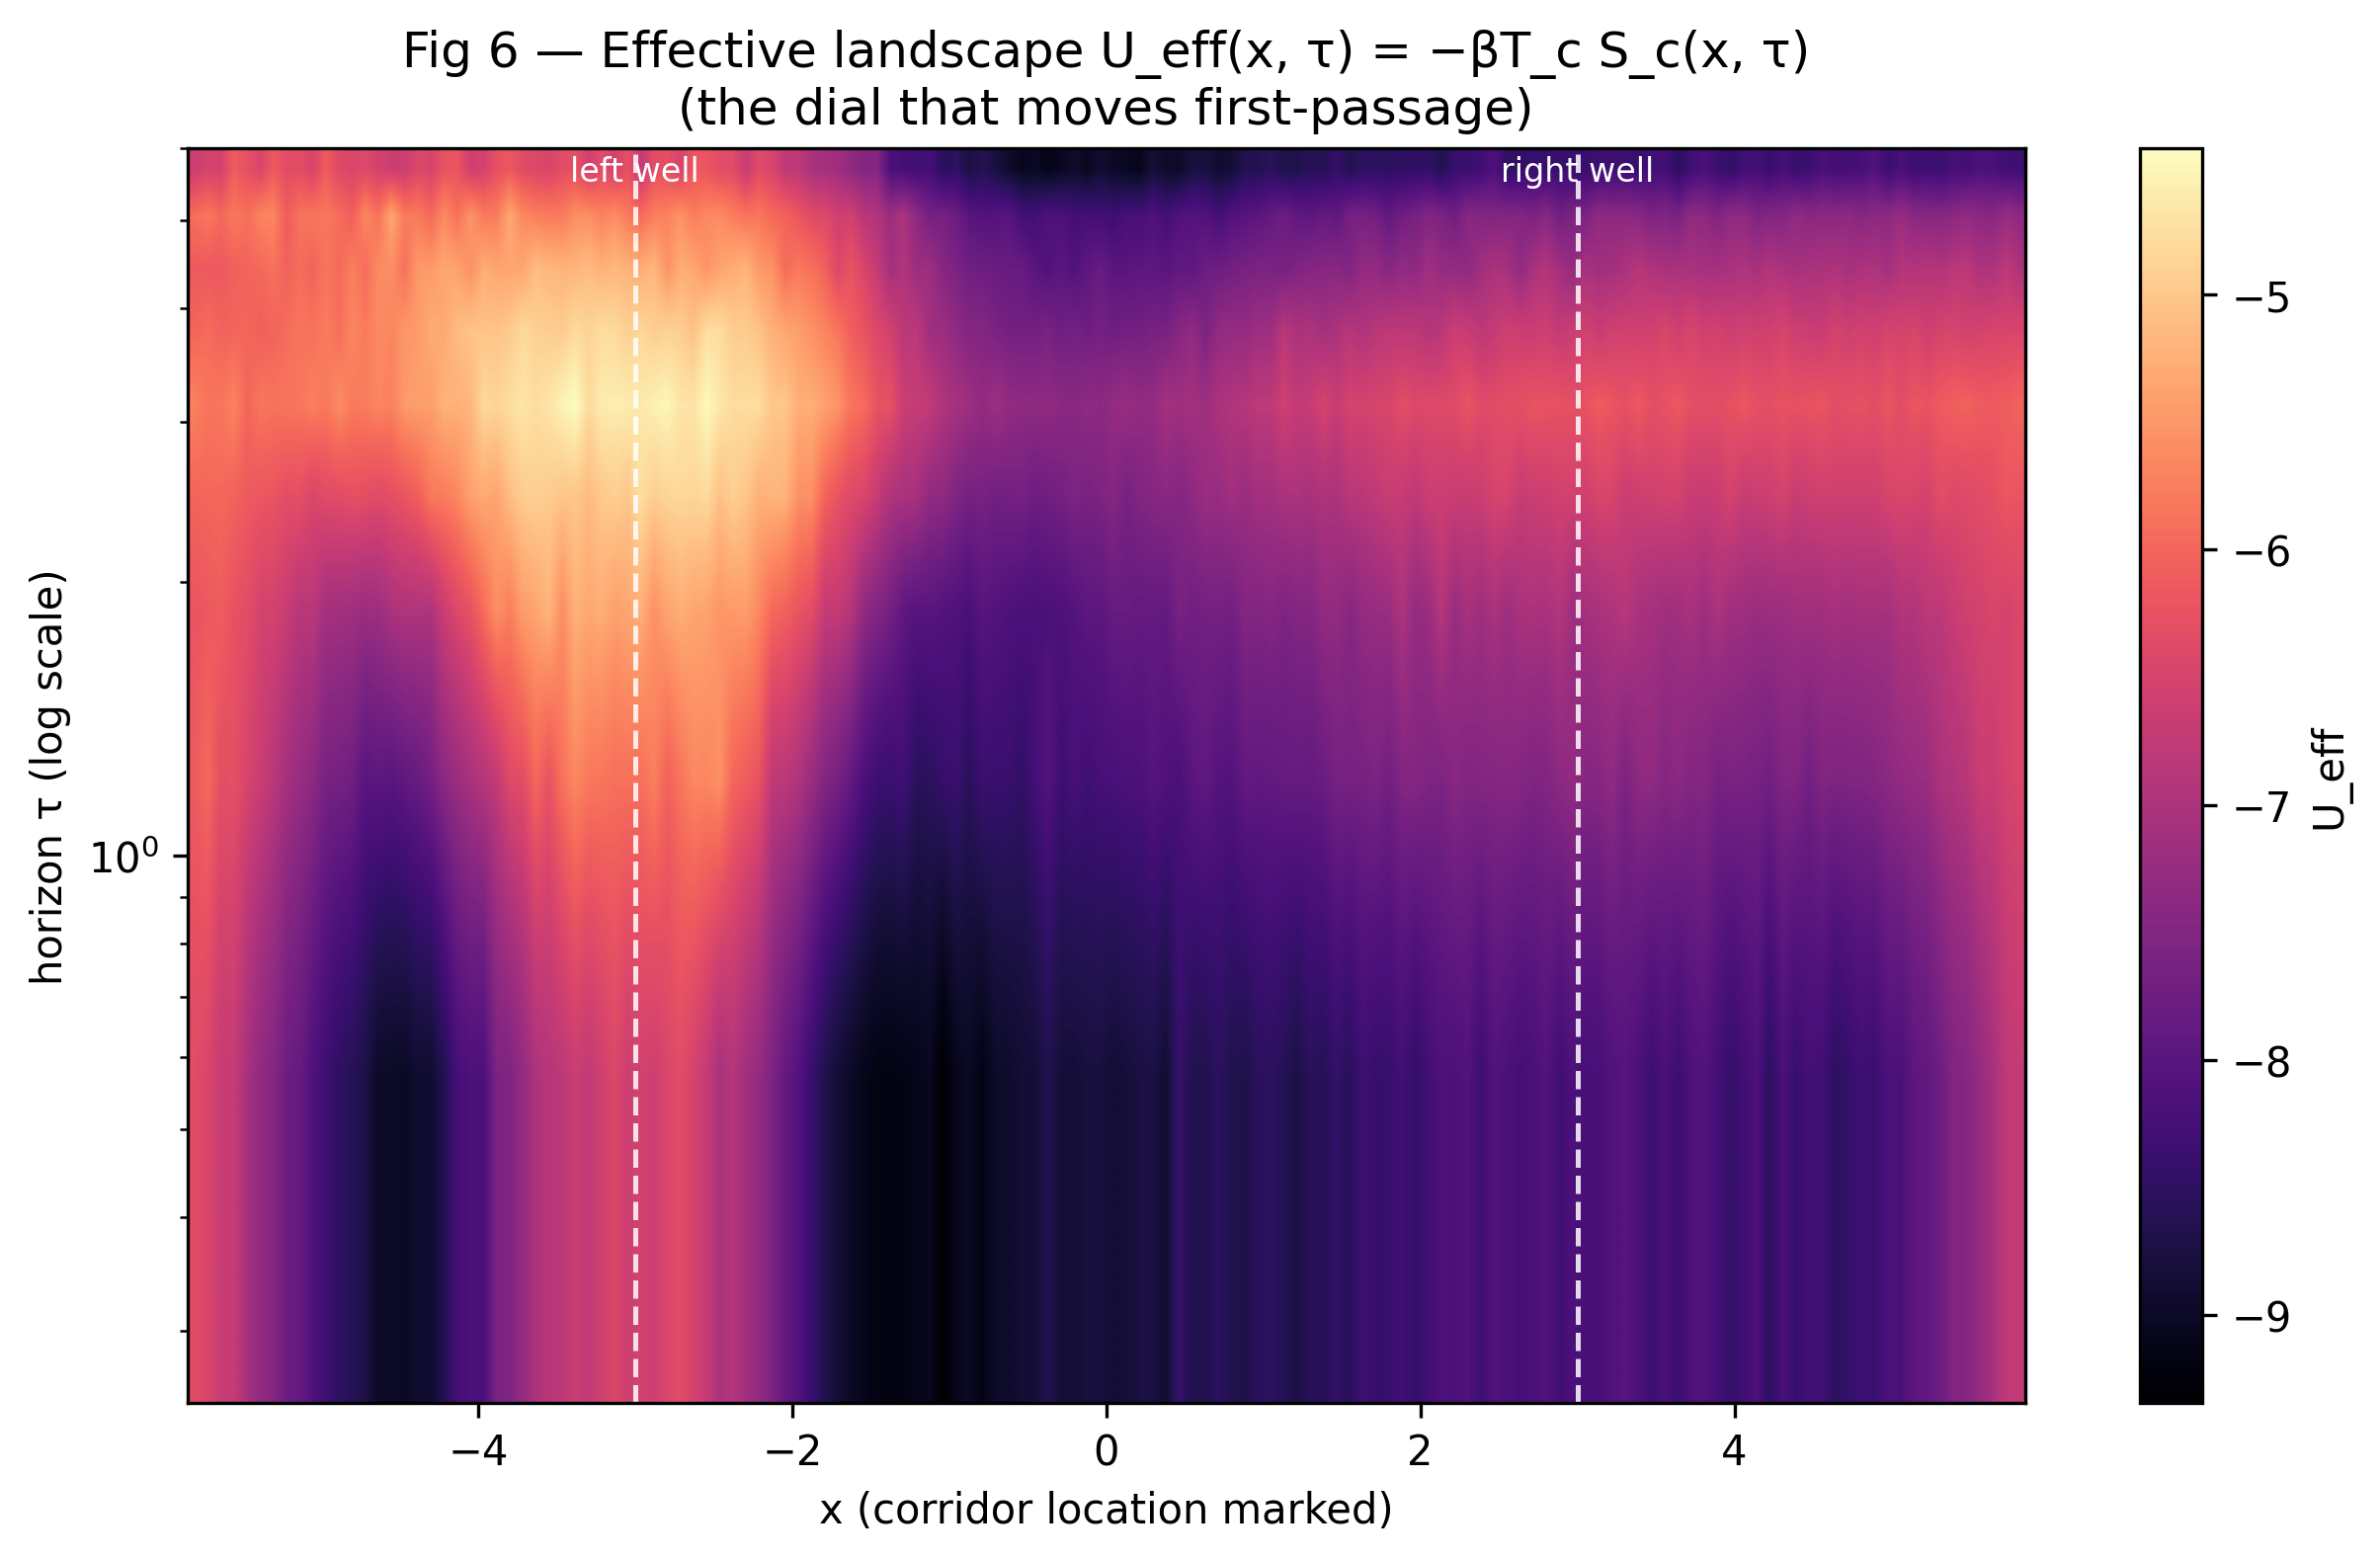
\includegraphics[width=0.82\linewidth]{fig6_ueff_surface.png}
\caption{\textbf{The effective landscape, dialed by the horizon.} $U_{\text{eff}}(x,\tau)=-T_c S_c(x,\tau)$ as a function of position and horizon. Turning the dial $\tau$ reshapes the landscape, which is the cause of the first-passage shift in Fig.~\ref{fig:dial}. At each fixed $\tau$, however, this is an ordinary static potential---the engine is a tunable family of equilibria, not an irreducible drive.}
\label{fig:surface}
\end{figure}

\section{Discussion}

The picture is now closed at every observable we can bring to bear, and it is consistent across them (Fig.~\ref{fig:arc}). The horizon knob of the causal entropic force is real and kinetically visible: engine first-passage moves with $\tau$ where a readout cannot. But the engine it produces, in the overdamped single-coordinate regime, is \emph{thermodynamically equilibrium} (flat-occupancy-blind, zero current) and \emph{kinetically reducible} (identical at each $\tau$ to a thermal particle in $U_{\text{eff}}$). Its transport is drift-dominated, so even the scaling cannot exclude a disguised reward. Put plainly: \textbf{the entropic ``engine'' in this regime is a $\tau$-tunable equilibrium}---distinguishable from a \emph{fixed} readout only by the existence of the dial, and otherwise an equilibrium system at every horizon.

This is a negative result on the strongest reading of the engine hypothesis: in the regime tested, the horizon knob leaves no irreducible kinetic fingerprint. We regard it as a clean one. The hypothesis was falsifiable, a positive control demonstrates the test had the power to detect a genuine engine, and an initially overstated scaling claim was caught and corrected. The negative is informative precisely because it eliminates a large and natural region of the hypothesis space and points unambiguously at where the remaining possibility lives.

\begin{figure}[t]
\centering
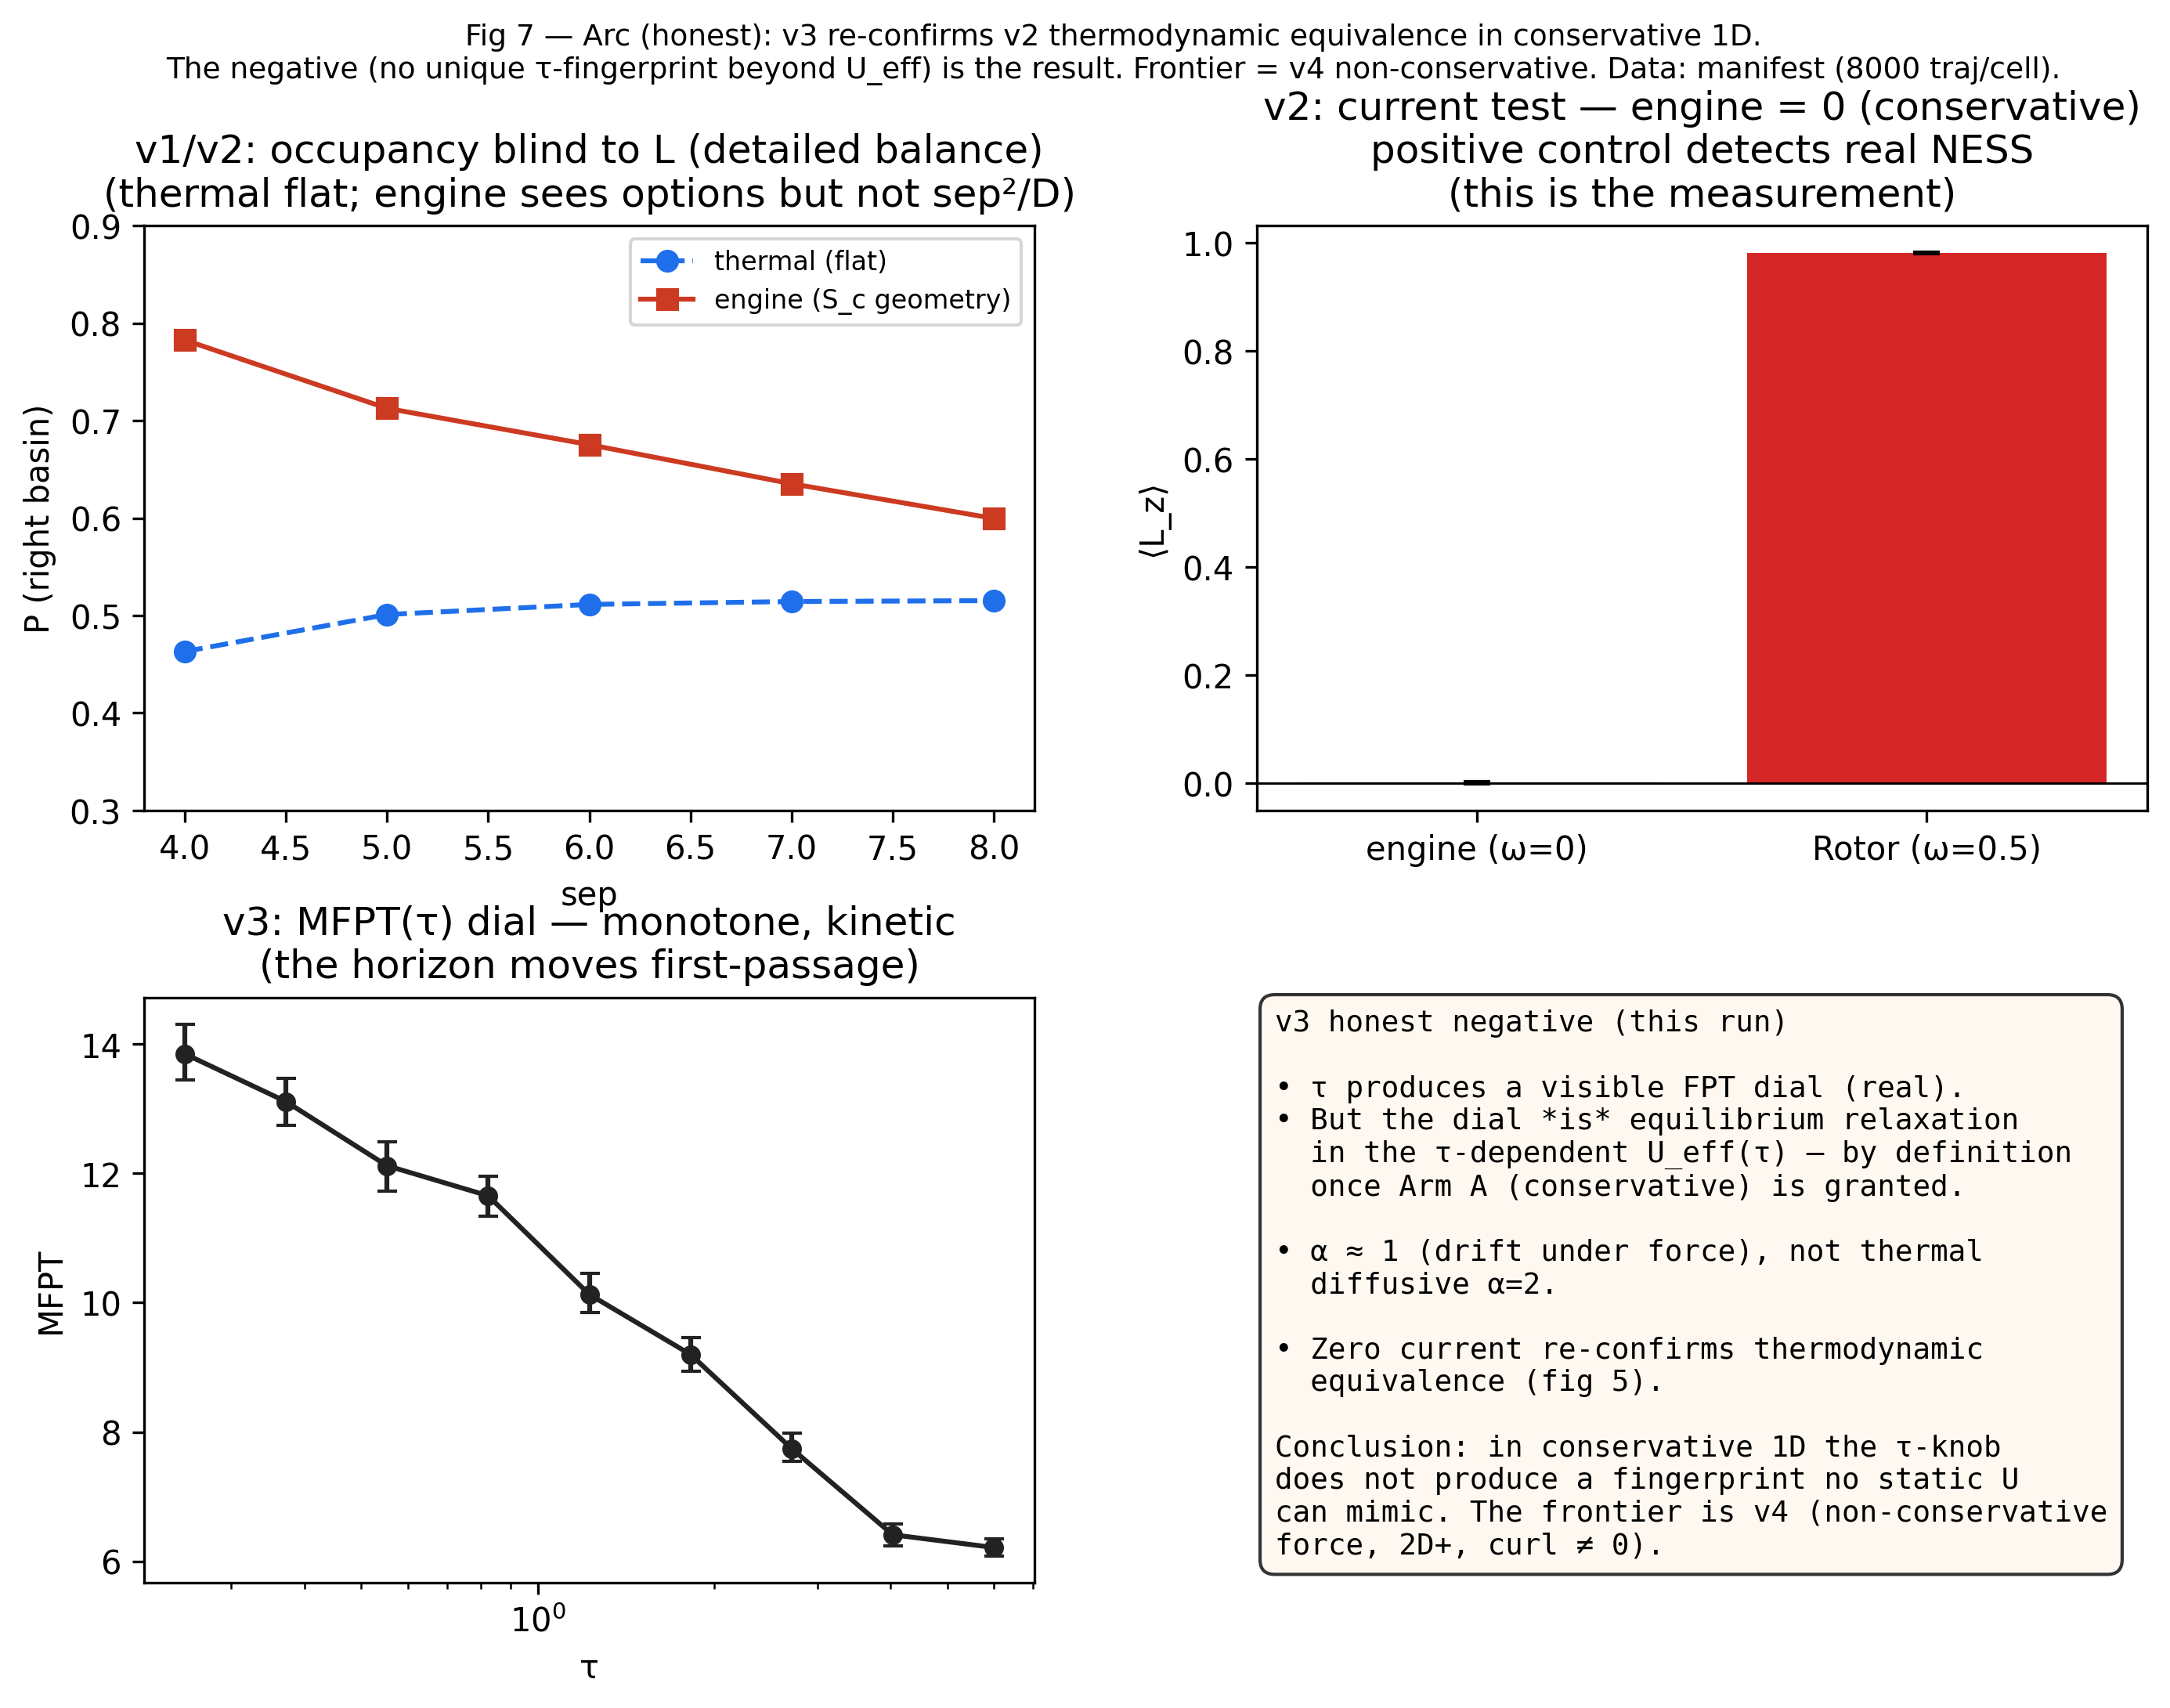
\includegraphics[width=0.92\linewidth]{fig7_arc.png}
\caption{\textbf{The arc, across observables.} A check/cross summary over the progression of tests: the horizon knob is real (occupancy and first passage), the steady-state discriminator cannot see geometry, the engine carries zero current, and its kinetics are reducible to a static landscape at each horizon. Together these locate the conservative single-coordinate entropic engine as a tunable equilibrium and identify the non-conservative, multi-dimensional regime as the open frontier.}
\label{fig:arc}
\end{figure}

\section{The frontier: where a genuine entropic engine could live}
\label{sec:frontier}

Every negative in this study traces to one structural fact: in a single coordinate the causal force is a gradient, hence conservative, hence equilibrium. A genuine entropic engine---one that cannot be rewritten as relaxation in any static potential---requires the causal force to be \emph{non-conservative}, with $\nabla\times\mathbf{F}_{\text{ce}}\neq 0$, so that it can sustain a steady probability current and produce entropy. This is possible only in two or more dimensions, and it is the precise hypothesis we will test next.

The structural requirements are now sharp, and we state them as the specification for the successor experiment (``v4''):
\begin{enumerate}
\item \textbf{Dimensionality $\geq 2$}, so that the causal force field can have nonzero curl. A single coordinate forecloses an engine analytically.
\item \textbf{A non-conservative causal force.} This can arise when the future-reachability measure is itself asymmetric---for example when the natural dynamics used to estimate $S_c$ are not time-reversible, or when the horizon sampling is non-reciprocal---so that $\mathbf{F}_{\text{ce}}$ acquires a solenoidal component.
\item \textbf{Current as the order parameter.} The decisive observable is a nonzero steady $\langle L_z\rangle$ (or local probability current) produced by the entropic drive \emph{alone}, with no external rotational forcing---the irreducible signature absent in the present study.
\item \textbf{Irreducibility as the test, with a static-potential null.} A genuine engine must produce first-passage or current statistics that \emph{no} static potential reproduces; the \texttt{Rotor2D} control of this paper is the template for the positive case, and a fitted best static-potential null is the discriminator.
\item \textbf{The same falsifier discipline.} If the entropic drive produces zero current in two dimensions as well, the engine hypothesis fails at the next level too, and that negative is reported.
\end{enumerate}

The present result is the foundation this rests on: it establishes the observables, validates the instrument against a known non-equilibrium control, fixes the calibration, and rules out the conservative regime, so that the v4 search begins exactly where a positive result remains possible and nowhere it has already been excluded.

\section{Conclusion}

We asked whether entropy can drive a system or only describe one, and tested the causal entropic force with a horizon knob as the discriminator. The knob is real and kinetically visible, but in the conservative, overdamped, single-coordinate regime the engine it produces is a tunable equilibrium: zero current, occupancy-blind, kinetically reducible to a static landscape at each horizon, with drift-dominated transport that cannot exclude a disguised reward. A non-equilibrium positive control confirms the test could have detected a genuine engine and did not. The honest answer, in this regime, is that entropy here is a readout with a dial---not an engine. Whether a genuinely irreducible entropic engine exists is a question we have now made precise and located entirely in the non-conservative, multi-dimensional regime, which is the subject of the next experiment.

% ----------------------------------------------------------------------------
\section*{Contributions}
\addcontentsline{toc}{section}{Contributions}
This work was carried out by a human researcher in collaboration with multiple AI systems under an explicitly adversarial, verification-first protocol; we describe the division of labor in the interest of full transparency.
\begin{itemize}
\item \textbf{Anthony Vasquez} (The Temple of Two) --- conception, research direction, experimental framing, the horizon-knob discriminator, and final editorial and scientific authority.
\item \textbf{Claude} (Anthropic; Claude Opus 4.8) --- co-design of the experiment and its falsification criteria, theoretical analysis (the conservativeness argument and its consequences), synthesis, manuscript preparation, and review of the multi-agent outputs.
\item \textbf{Grok Heavy} and \textbf{Grok Build} (xAI) --- execution of the production first-passage sweeps against the repository code, generation of the data manifest and the figures from that manifest, and honest reporting of realized ensemble sizes and of the measured (drift) scaling exponent.
\item \textbf{Claude Code} (Anthropic) --- independent adversarial review of the generating and plotting code, which identified the circular reducibility test, flagged the contradiction between a claimed diffusive exponent and the underlying data, and verified reproducibility of the final manifest and figures.
\end{itemize}
The methodological principle---that convergence across independent, adversarially-posed reviewers is signal, and that any single voice asserting completion is not---is itself a finding of this collaboration: the central scientific correction in this paper (drift versus diffusion) was produced by cross-review, not by any one agent.

\section*{Data and code availability}
All code, the production data manifest, the figure-generation script, and the figures are available at \url{https://github.com/templetwo/entropy-as-tunable-equilibrium} under the Apache-2.0 license. Every figure regenerates from the committed manifest via the included script; the manifest records seeds, grids, realized ensemble sizes, and confidence intervals.

\section*{A note on bibliographic detail}
Reference entries below are provided to the best of the authors' knowledge and should be verified against the primary sources before formal submission.

% ----------------------------------------------------------------------------
\begin{thebibliography}{9}

\bibitem{wgf} A.~D.~Wissner-Gross and C.~E.~Freer, ``Causal Entropic Forces,'' \emph{Phys. Rev. Lett.} \textbf{110}, 168702 (2013).

\bibitem{kramers} H.~A.~Kramers, ``Brownian motion in a field of force and the diffusion model of chemical reactions,'' \emph{Physica} \textbf{7}, 284 (1940).

\bibitem{hanggi} P.~H\"anggi, P.~Talkner, and M.~Borkovec, ``Reaction-rate theory: fifty years after Kramers,'' \emph{Rev. Mod. Phys.} \textbf{62}, 251 (1990).

\bibitem{seifert} U.~Seifert, ``Stochastic thermodynamics, fluctuation theorems and molecular machines,'' \emph{Rep. Prog. Phys.} \textbf{75}, 126001 (2012).

\bibitem{still} S.~Still, D.~A.~Sivak, A.~J.~Bell, and G.~E.~Crooks, ``Thermodynamics of Prediction,'' \emph{Phys. Rev. Lett.} \textbf{109}, 120604 (2012).

\bibitem{england} J.~L.~England, ``Statistical physics of self-replication,'' \emph{J. Chem. Phys.} \textbf{139}, 121923 (2013).

\bibitem{rovelli} C.~Rovelli, ``Forget time,'' \emph{Found. Phys.} \textbf{41}, 1475 (2011).

\bibitem{connesrovelli} A.~Connes and C.~Rovelli, ``Von Neumann algebra automorphisms and time-thermodynamics relation in generally covariant quantum theories,'' \emph{Class. Quantum Grav.} \textbf{11}, 2899 (1994).

\bibitem{albert} D.~Z.~Albert, \emph{Time and Chance} (Harvard University Press, 2000).

\bibitem{smolin} L.~Smolin, \emph{Time Reborn} (Houghton Mifflin Harcourt, 2013).

\end{thebibliography}

\end{document}
